\section{Teilaufgabe 5}
\begin{aufgabe}
    Zeichnen Sie das asymptotische Nyquist-Diagramm von $P_1(s)$.
\end{aufgabe}
\begin{figure}[h!]
    \centering
    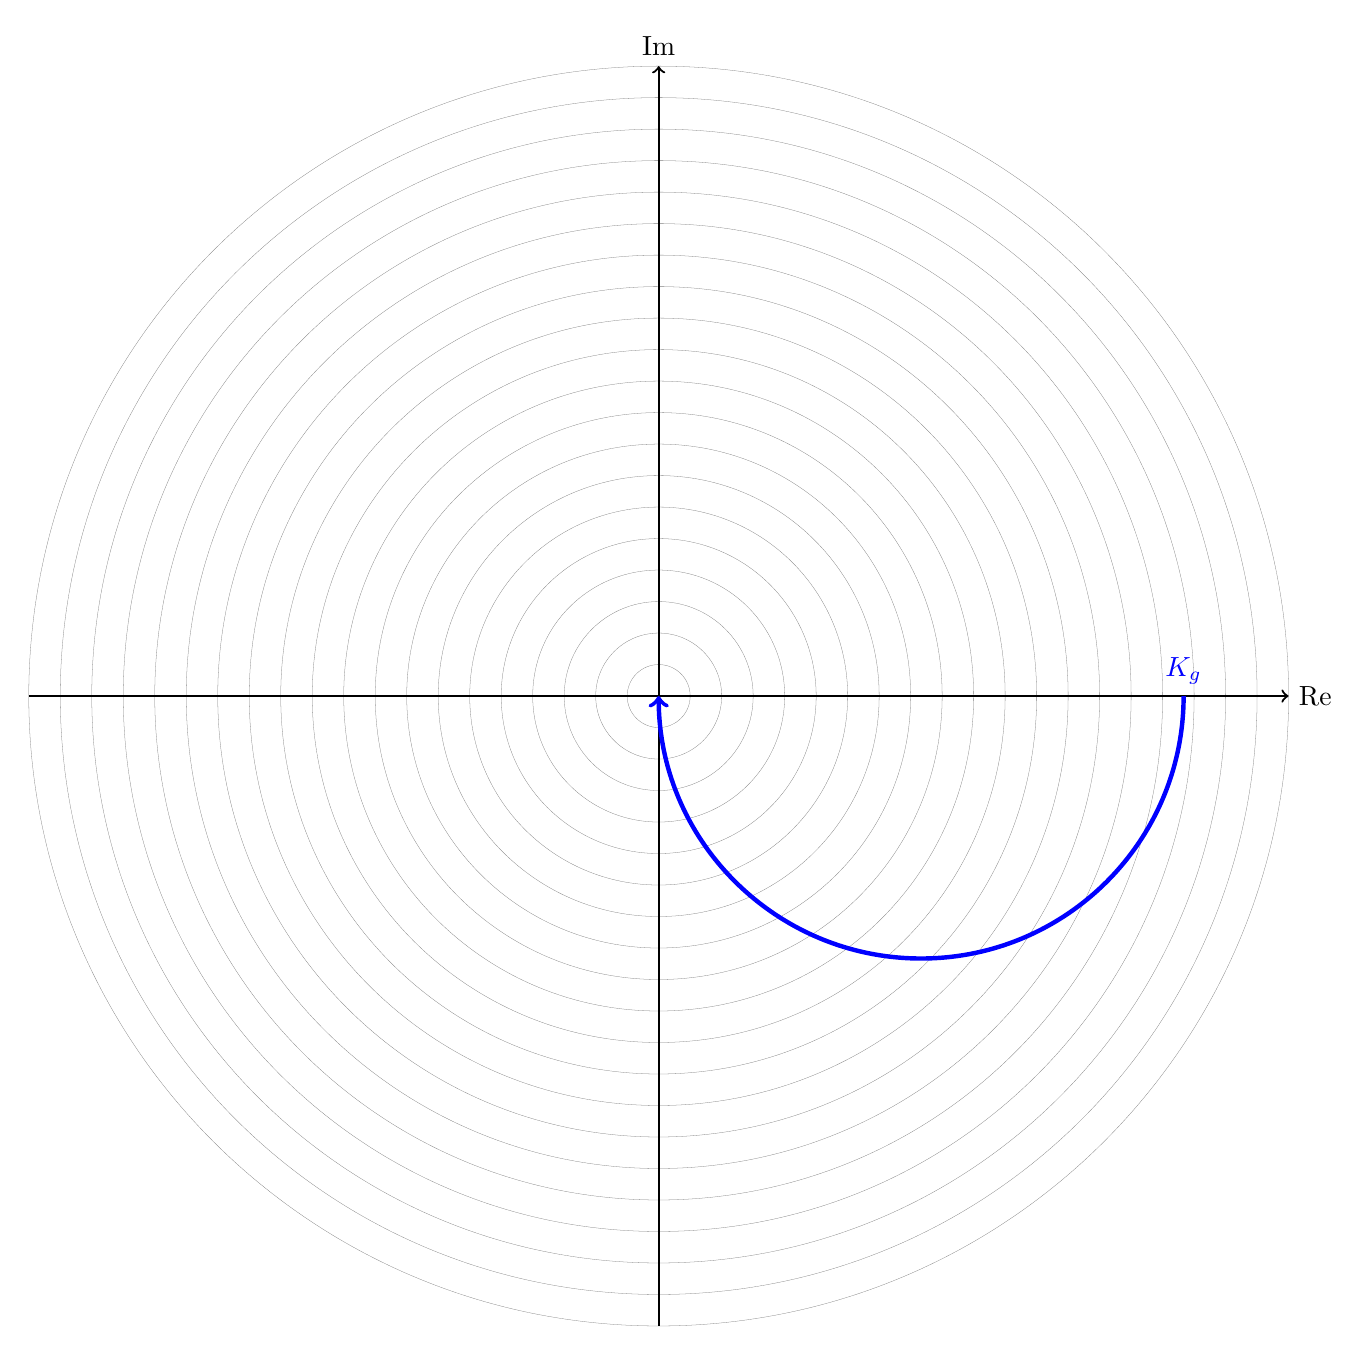
\begin{tikzpicture}[scale=0.4]
        \foreach \i in {0, 1, ..., 20}
        {
            \draw[ultra thin, gray] (\i,0)
                arc[radius=\i, start angle = 0, end angle = 360];
        }
        \draw[thick, ->] (-20, 0) -- (20, 0) node[right] {Re};
        \draw[thick, ->] (0, -20) -- (0, 20) node[above] {Im};
        \draw[ultra thick, blue, ->] (16.666667,0) node[above] {$K_g$}
            arc[radius=16.666667/2, start angle = 0, end angle = -180];
    \end{tikzpicture}
\end{figure}
